\documentclass[../../main.tex]{subfiles}

\begin{document}

\chapter{Results}

A number of experiments were conducted with two broad goals: verifying that at least some of the proposed options work on simplified abstract engineering environments, and proving that the proposed architecture has desirable qualities in more complex environments.
Some experiments were also carried out to visualise and explore the latent space mappings in an intuitive way.

\section{Approach verification}

\subsection{Distribution distance}

Due to the potential issues with minimising KL-divergence discussed in \S4.1.2, a highly simplified environment was devised in which the target distribution is known.
The target distribution was fixed as a standard normal distribution (constraints were not considered at this stage) and the generator's output distribution was modelled as a normal distribution whose mean and standard deviation were controllable parameters.

Although KL-divergence is analytically tractable for two normal distributions, it was estimated through sampling of the generated distribution as described in \S4.1.1.
Trained variables were initialised such that the standard deviation started at $1$, while the initial mean was varied.
\begin{figure}[H]
    \begin{center}
    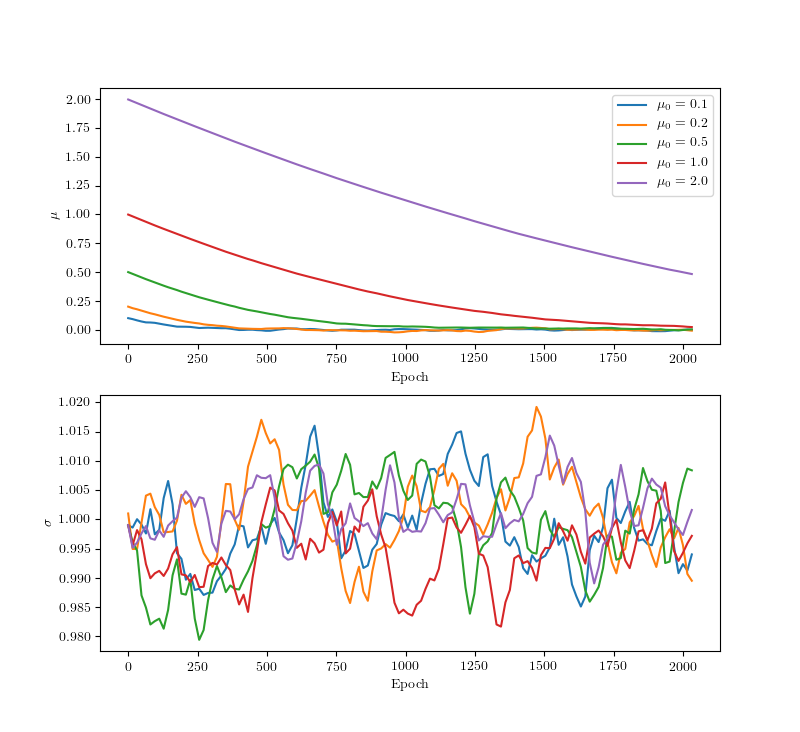
\includegraphics[width=\textwidth]{broadKLDivergence}
    \caption{
        Change in $\mu$ and $\sigma$ over time when training arbitrary normal distributions with different starting means to match the standard normal distribution. 
        Parameters were updated using the Adam optimisation algorithm to minimise KL-divergence, as estimated by taking samples from the varying distribution in batches of 64.
    }
    \label{fig:broadKLDivergence}
    \end{center}
\end{figure}
The mean $\mu$ and standard deviation $\sigma$ after each batch are shown in Figure \ref{fig:broadKLDivergence}.
Convergence does occur, but the time taken for the mean to approach $0$ appears to increase exponentially as the initial mean moves away from the target.
Two one-dimensional normal distributions whose means only differ by two and whose standard deviations are both one could still be considered to be quite close together, so the experiment was repeated with $\sigma=0.1$ for both distributions to better simulate disjoint distributions.
\begin{figure}[H]
    \begin{center}
    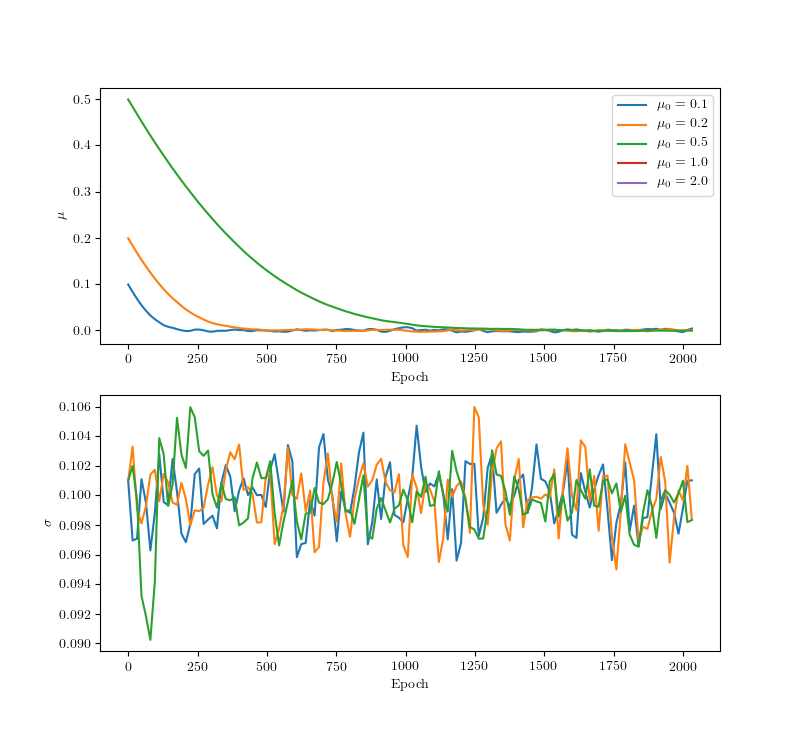
\includegraphics[width=\textwidth]{narrowKLDivergence}
    \caption{
        Change in $\mu$ and $\sigma$ over time when training arbitrary normal distributions with different starting means to match a normal distribution with $\mu=0$ and $\sigma=0.1$. 
        Parameters were updated using the Adam optimisation algorithm to minimise KL-divergence, as estimated by taking samples from the varying distribution in batches of 64.
    }
    \label{fig:narrowKLDivergence}
    \end{center}
\end{figure}
Figure \ref{fig:narrowKLDivergence} shows that the variables converge at approximately the same rate as when the standard deviation of the target distribution was $1$.
Missing, however, are the trend lines for $\mu_0=1.0$, $\mu_0=2.0$; both $\mu$ and $\sigma$ went to \url{NaN} after the first epoch.
This may well have been caused by an excessively large KL-divergence resulting in exploding gradients due to the limited precision of floating point numbers.

Changing the computation graph to use \url{float64} values instead of \url{float32} lends further evidence to this hypothesis, as increasing the precision allowed the $\mu=1.0,2.0$, $\sigma=0.1$ cases to be optimised without numerical errors (Figure \ref{fig:narrowKLDivergenceFloat64}).
Similarly, using 16-bit floating point values always resulted in \url{NaN} errors occurring.
\begin{figure}[H]
    \begin{center}
    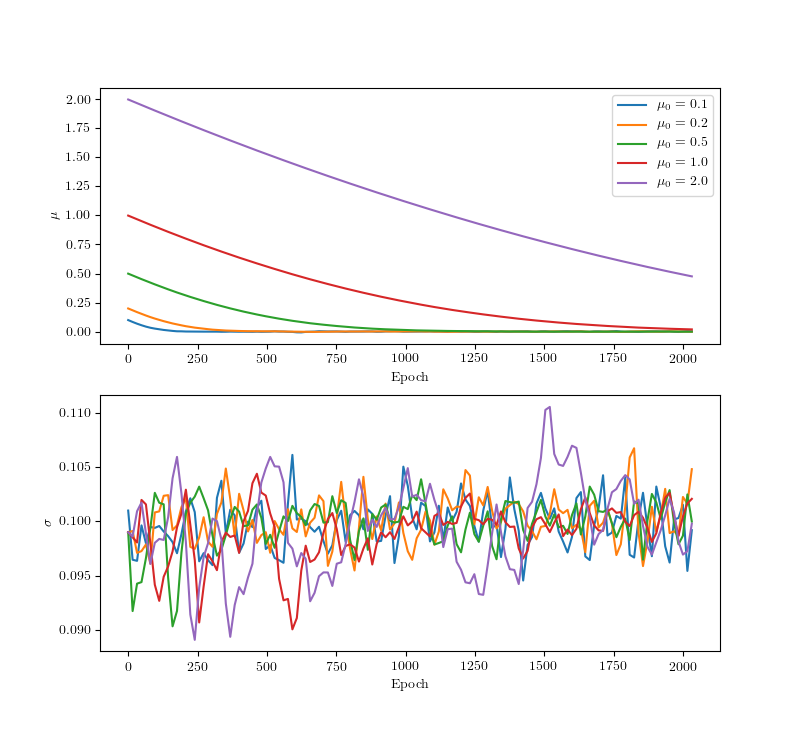
\includegraphics[width=\textwidth]{narrowKLDivergenceFloat64}
    \caption{
        Change in $\mu$ and $\sigma$ over time when training arbitrary normal distributions with different starting means to match a normal distribution with $\mu=0$ and $\sigma=0.1$. 
        Experimental parameters are the same as in Figure \ref{fig:narrowKLDivergence}, but with 64-bit floating point numbers as opposed to 32-bit.
    }
    \label{fig:narrowKLDivergenceFloat64}
    \end{center}
\end{figure}
It was therefore concluded that minimising KL-divergence is too inconsistent for practical use, as real distributions $-$ which are frequently disjoint $-$ would very likely cause numerical issues due to lack of the required precision.

\subsection{Precision proxy optimisation}

Potential issues with directly estimating the recall of one distribution with respect to another were discussed in \S4.3.
It was also hypothesised that optimising only for precision, $\hat{p}(g)$, would result in the generator sampling only a small subset of the viable solutions.

A short experiment was devised to prove that this is the case and hence that some other approximation of the recall would be needed.
A function modelling the probability of satisfaction for a solution in one dimension ($m=1$) was defined arbitrarily as:
$$h(c,s)=\sigma(20c-6)-\sigma(20c-14)$$
where
$$\sigma(x)=\frac{1}{1+e^{-x}}$$
and there is only one possible constraint for the sake of simplicity ($n=0$).
A graph of the constraint satisfaction function on $[-1, 1]$ is shown in Figure \ref{fig:sigmoidBumpFunction}.
Numerically integrating $h$ between $c=-1$ and $c=1$ gives an area of $~0.3999$, so the probability density function is $\hat{V}(c)(s)\approx2.5008\;h(c,s)$.
\begin{figure}[H]
    \begin{center}
    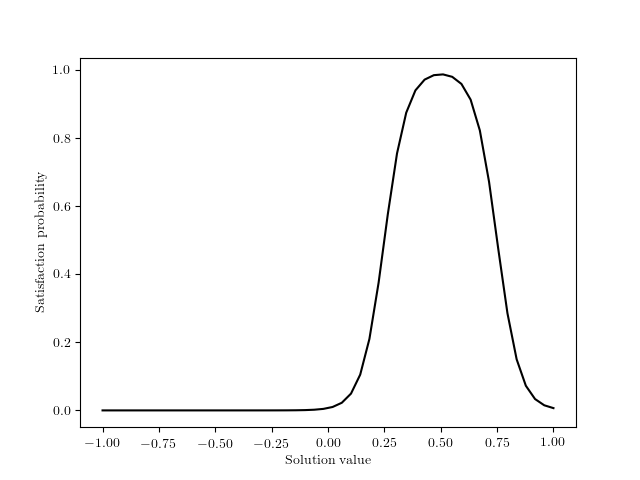
\includegraphics[width=\textwidth]{sigmoidBumpFunction}
    \caption{
        A test function estimating the probability that a solution $s$ satisfies a singular constraint $c$.
    }
    \label{fig:sigmoidBumpFunction}
    \end{center}
\end{figure}
Optimising the generator against $h(c,s)$ for the precision proxy defined in \S4.2.1 consistently yields a distribution of generated solutions displayed in Figure \ref{fig:sigmoidBumpHistogram}.
Only considering precision and disregarding recall has clearly produced a mapping which is of no use: it always maps to the same point in spite of the fact that around $15\%$ of the solution space has a constraint satisfaction probability above $0.9$.
\begin{figure}[H]
    \begin{center}
    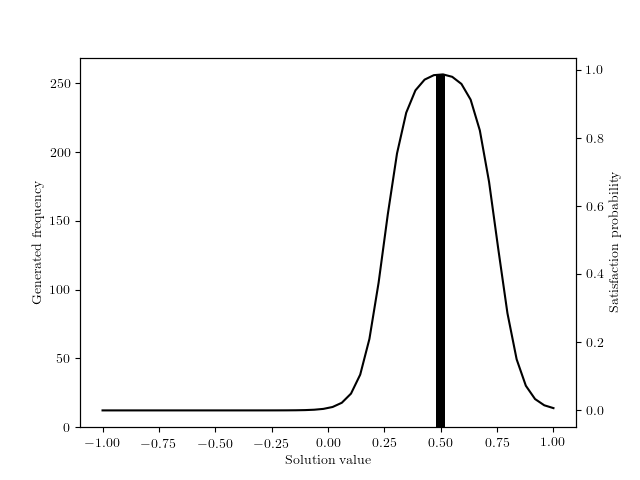
\includegraphics[width=\textwidth]{sigmoidBumpHistogram}
    \caption{
        Distribution of generated solutions compared to the constraint satisfaction function against which the generator was trained, in the form of a histogram consisting of 256 samples.
        The generator had two hidden layers, each with 8 leaky-ReLU activated units, and a single $\tanh$ output unit.
    }
    \label{fig:sigmoidBumpHistogram}
    \end{center}
\end{figure}
This issue becomes even more pronounced when the constraint satisfaction function is altered to have two distinct modes (Figure \ref{fig:sigmoidBumpHistogramBimodal}).
$$h(c,s)=\sigma(20c-6)-\sigma(20c-14)+\sigma(20c+6)-\sigma(20c+14)$$
While a very high precision is obtained, with all generated solutions having a satisfaction probability of $~96\%$, optimising solely for precision fails entirely to encapsulate the bimodality of the constraint satisfaction function even in such a simple environment, confirming that optimisation must take recall into consideration for satisfactory results.
\begin{figure}[H]
    \begin{center}
    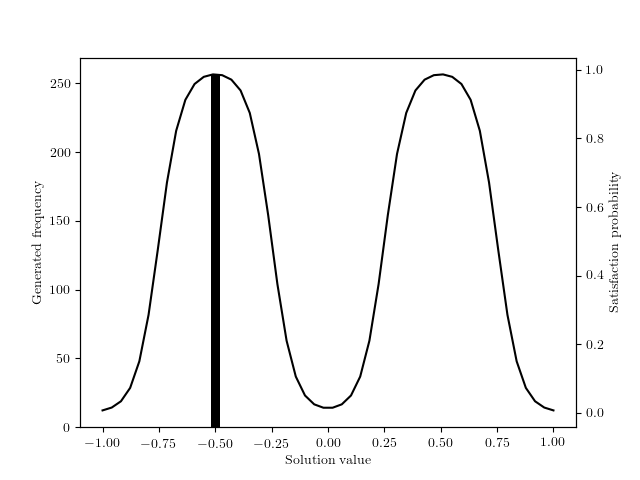
\includegraphics[width=\textwidth]{sigmoidBumpHistogramBimodal}
    \caption{
        Distribution of generated solutions compared to a bimodal constraint satisfaction function against which the generator was trained, in the form of a histogram consisting of 256 samples.
        The generator architecture is the same as that used in Figure \ref{fig:sigmoidBumpHistogram}.
    }
    \label{fig:sigmoidBumpHistogramBimodal}
    \end{center}
\end{figure}

\subsection{Pretraining}

In the absence of a recall proxy, it was suggested that the generator be pretrained to ensure that its initial distribution covers as wide a range of the solution space as possible.
This is based on two suppositions: that the generator initially only takes samples from an isolated region of the solution space; and that a more general distribution would explore multiple high-satisfaction regions of the solution space, thereby capturing a multimodal distribution even when optimising only for precision.
The generator's architecture remained the same as that used in \S6.1.2, and the bimodal constraint satisfaction function from the latter half of that section was also used.

That the first assumption is true is confirmed trivially by taking samples from the generator before training (Figure \ref{fig:initialisedGenerator}).
Glorot initialisation, a common method of initialising the weights of neural networks, was used to initialise the generator's network weights.
\begin{figure}[H]
    \centering
    \begin{subfigure}[a]{1.\textwidth}
        \centering
        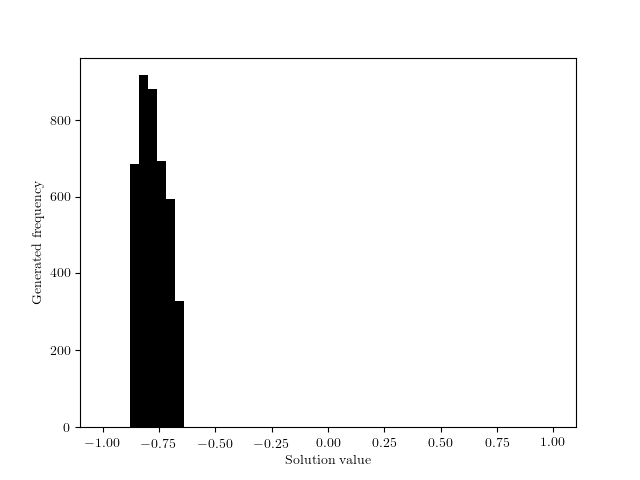
\includegraphics[width=0.6\textwidth]{initialisedGenerator1}
    \end{subfigure}
    \begin{subfigure}[a]{1.\textwidth}
        \centering
        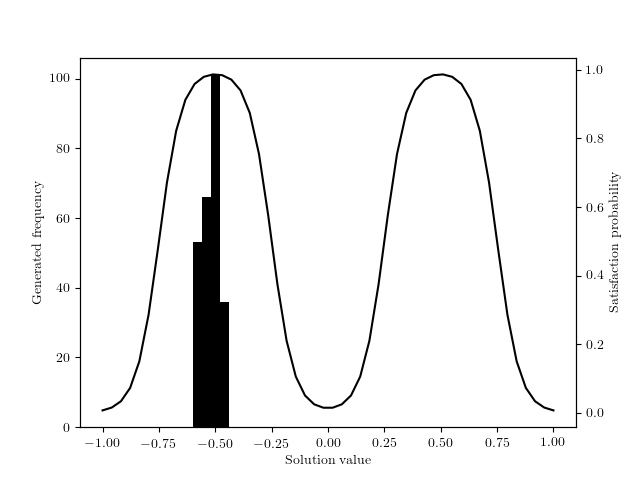
\includegraphics[width=0.6\textwidth]{initialisedGenerator2}
    \end{subfigure}
    \begin{subfigure}[a]{1.\textwidth}
        \centering
        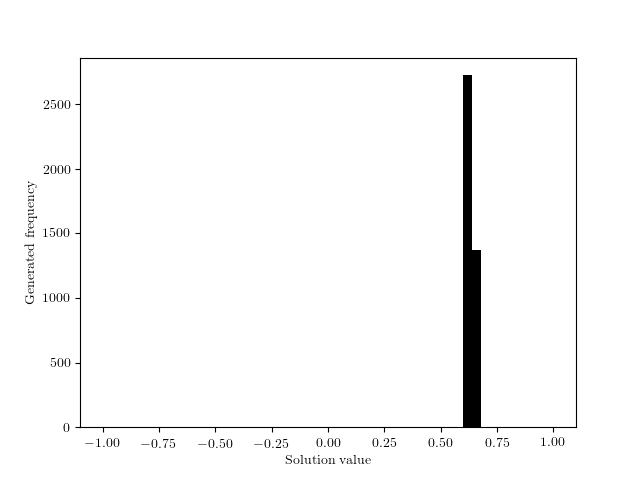
\includegraphics[width=0.6\textwidth]{initialisedGenerator3}
    \end{subfigure}
    \caption{
        Generated distribution immediately after network initialisation for three different seeds using a larger batch size of 4096.
    }
\label{fig:initialisedGenerator}
\end{figure}
Pretraining is performed in the same way as normal training, but instead of minimising the precision loss, one of the spread losses $q_\text{id}$ or $q_\text{sep}$ is minimised.
Because the spread is a subjective quality which cannot obviously be objectively measured, the success of each spread metric will be judged on whether it enables the generator to learn both modes of the viable set simultaneously.
That spread function will then be used in further experiments.

Below are examples of typical generated viable sets after pretraining with each spread metric.
Identity spread (Figure \ref{fig:identitySpread}) was trained with a batch size of 4096, while separation spread (Figure \ref{fig:separationSpread}) was trained with a smaller batch size of 256 to prevent excessive computations.
The target spread was set to $q_\text{target}=1$, such that the desired mean distance between sampled solutions is equal to $1$.
\begin{figure}[H]
    \begin{center}
    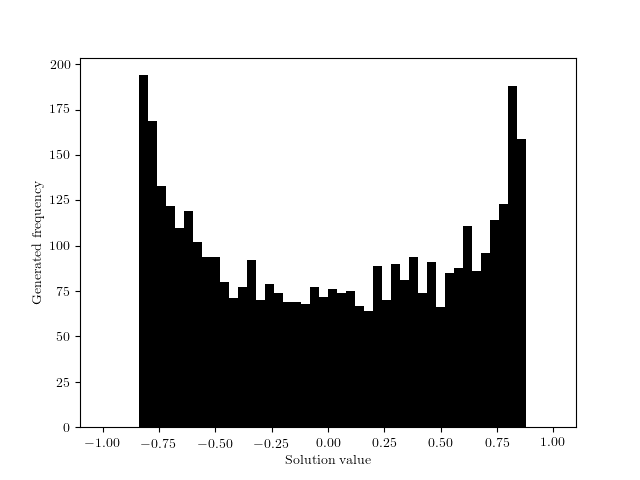
\includegraphics[width=\textwidth]{identitySpread}
    \caption{
        Generator output distribution after pretraining until convergence using the identity spread loss $q_\text{id}$ and a batch size of 4096.
    }
    \label{fig:identitySpread}
    \end{center}
\end{figure}

\begin{figure}[H]
    \begin{center}
    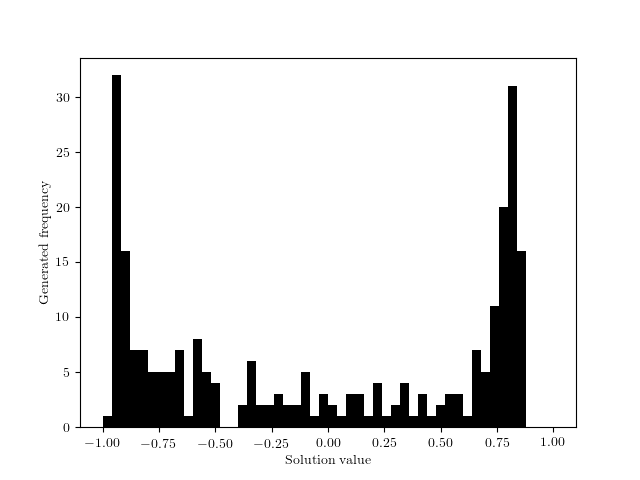
\includegraphics[width=\textwidth]{separationSpread}
    \caption{
        Generator output distribution after pretraining until convergence using the separation spread loss $q_\text{sep}$ with a target spread of $q_\text{target} = 1$ on batches of size 256.
    }
    \label{fig:separationSpread}
    \end{center}
\end{figure}
Both spread metrics show signs of causing the generator to explore a far greater proportion of the solution space than immediately after initialisation, but also have a tendency to over-explore the boundaries.
This effect is much more pronounced with $q_\text{sep}$.
The true success of each metric, however, is determined by the generator's ability to find different nodes when precision is optimised after pretraining.
\begin{figure}[H]
    \begin{center}
    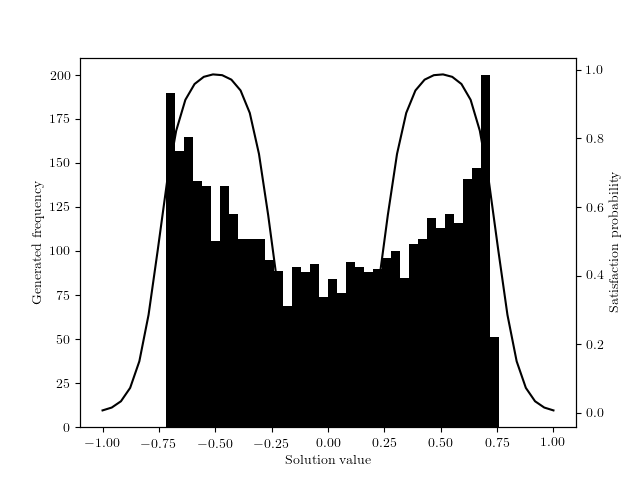
\includegraphics[width=\textwidth]{identityThenPrecision}
    \caption{
        Generator output distribution after pretraining until convergence using the identity spread loss $q_\text{id}$ and a batch size of 4096, then trained to maximise precision for a further 8096 batches.
    }
    \label{fig:identityThenPrecision}
    \end{center}
\end{figure}

\begin{figure}[H]
    \begin{center}
    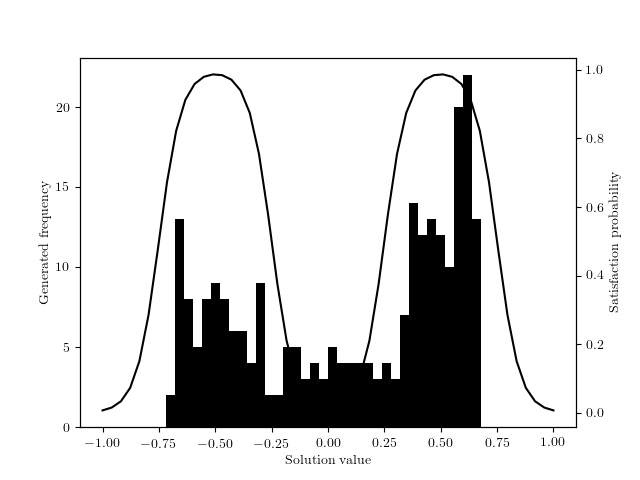
\includegraphics[width=\textwidth]{separationThenPrecision}
    \caption{
        Generator output distribution after pretraining until convergence using the separation spread loss $q_\text{sep}$ with a target spread of $q_\text{target} = 1$ on batches of size 256, followed by training to maximise precision on another 512 batches.
    }
    \label{fig:separationThenPrecision}
    \end{center}
\end{figure}
Comparing Figure \ref{fig:sigmoidBumpHistogramBimodal} to Figures \ref{fig:identityThenPrecision} and \ref{fig:separationThenPrecision} it is clear that the generator's ability to detect multiple modes is greatly enhanced by pretraining to maximise spread.
This comes at a cost, however; while the generator pretrained on $q_\text{id}$ samples in roughly equal proportions from both modes, it also frequently samples solutions from between the modes which are unlikely to satisfy the constraint.
Because both metrics have similar results but separation spread takes longer to train, the identity spread will be used in further experiments unless the latent space is required to have a different dimension to the solution space.

\subsection{Maximising precision and spread}

It was observed while training on precision after pretraining on spread that early stopping was required to prevent the generator from falling back into a unimodal distribution.
One possibility is, after pretraining, to minimise a weighted sum of precision and spread loss, as if the spread loss were a proxy for the recall of the learned viable distribution.
Using the identity spread, this is semantically valid: $q_\text{id}$ penalises the distance movement of probability mass between the latent and solution spaces, thereby providing an incentive to the generator to seek out areas of high satisfaction probability which are more local.

Figure \ref{fig:identityAndPrecision} shows the learned viable distribution after pretraining on identity spread, then training to minimise the sum of precision and identity spread loss ($w=1$) until convergence.
\begin{figure}[H]
    \begin{center}
    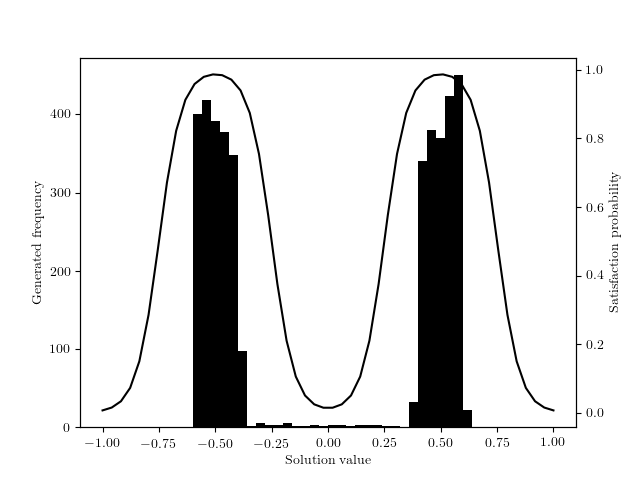
\includegraphics[width=\textwidth]{identityAndPrecision}
    \caption{
        Generator output distribution after pretraining as in Figure \ref{fig:identityThenPrecision}, followed by training to maximise the sum of precision and ideneity spread until convergence.
    }
    \label{fig:identityAndPrecision}
    \end{center}
\end{figure}
This is clearly a result superior to any obtained previously, with the generator sampling both modes, and almost always in regions with a satisfaction probability above $0.8$.
Solutions less likely to satisfy the constraint are almost never sampled.

\subsection{Constraint embeddings}

The only part of the proposed architecture that has yet to be verified is the insertion of constraints in an embedded form at the output layer of the generator.
This is achieved using a generalised alteration of the constraint satisfaction function used in \S6.1.3 such that the position of each peak is controlled by one dimension of the constraint.
Code used to construct this function inside a Tensorflow computation graph can be found in the appendix.
% Tensorflow was used to map the dimensions of the constraint vector onto this function, simulating a constraint satisfaction function learned by the discriminator:
% \begin{lstlisting}[language=Python]
% import tensorflow as tf

% constraint_dimension = 2

% def constraint_satisfaction_function(
%     solution_input, constraint_input
% ):
%     tiled_solution = tf.tile(
%         solution_input, [1, constraint_dimension]
%     )
%     summed_output = tf.reduce_mean(
%         sigmoid_peak(
%             tiled_solution, constraint_input
%         ), axis=1
%     )
%     return tf.reshape(
%         summed_output, [tf.shape(summed_output)[0], 1]
%     )

% def sigmoid_peak(
%     x,
%     offset,
%     width=5.0,
%     thickness=0.05,
%     height_scale=1.0
% ):
%     """Produces an individual peak centred on x."""
%     after_offset = (x - offset) / thickness
%     return height_scale * (
%         tf.sigmoid(after_offset + width) - \
%             tf.sigmoid(after_offset - width)
%     )
% \end{lstlisting}
The generator was trained to minimise a weighted sum of precision and identity spread (as a recall proxy) for 150 epochs of 20,000 steps each; a recall proxy weight of $0.7$ was used for these figures.
The generator had two hidden layers while both the weight and bias embedder had one hidden layer, with every hidden layer consisting of 32 leaky-ReLU units.
Constraints were mapped into a $10$-dimensional embedding vector.
All output layers were also leaky-ReLU activated, with the exception of the generator's output, which was tanh activated.

Generally, the generator was able to learn to adapt its learned viable distribution to account for the differences in the constraint satisfaction function.
Not only was it often able to distinguish between two modes, but also adjusted its mapping appropriately when the two peaks were near each other and so merged into one mode.
\begin{figure}[H]
    \centering
    \begin{subfigure}[a]{1.\textwidth}
        \centering
        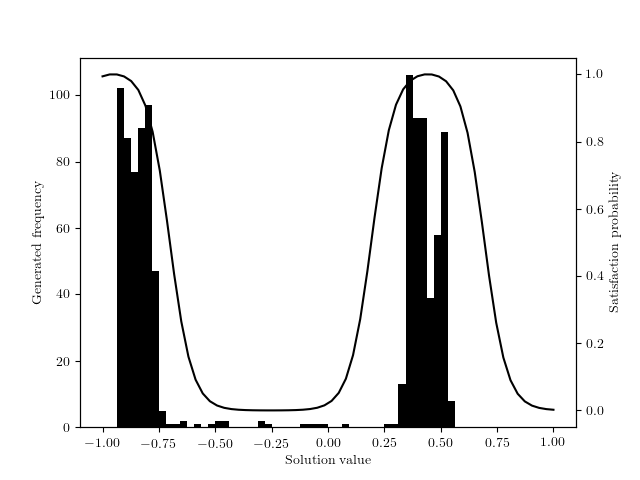
\includegraphics[width=0.6\textwidth]{embeddedConstraint1}
    \end{subfigure}
    \begin{subfigure}[a]{1.\textwidth}
        \centering
        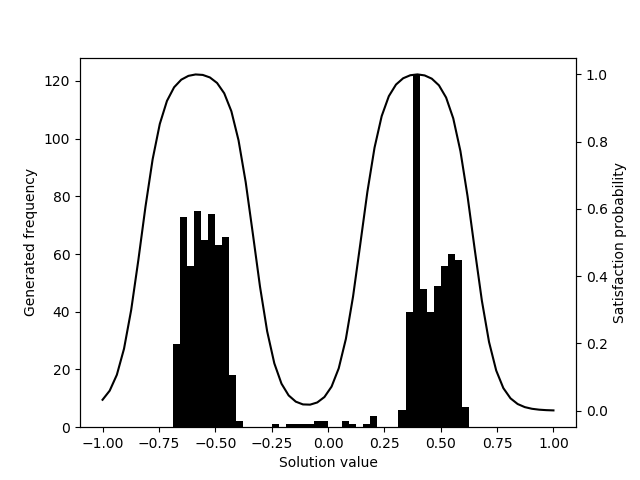
\includegraphics[width=0.6\textwidth]{embeddedConstraint2}
    \end{subfigure}
    \begin{subfigure}[a]{1.\textwidth}
        \centering
        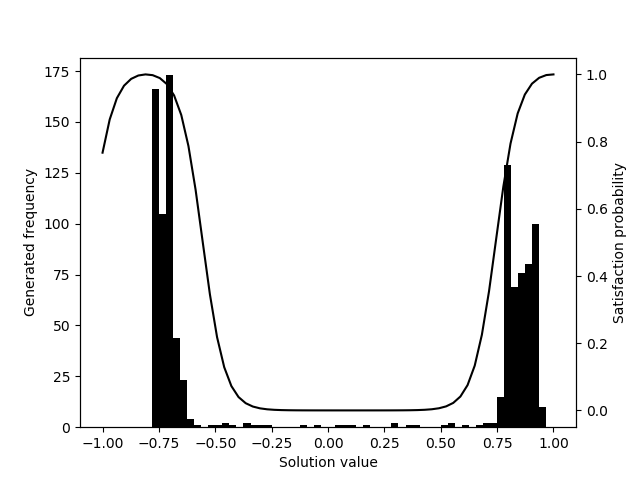
\includegraphics[width=0.6\textwidth]{embeddedConstraint5}
    \end{subfigure}
    \caption{
        Examples of a generator learning to adjust its mapping to changing constraints.
    }
\label{fig:embeddedConstraintsBimodal}
\end{figure}
Occasionally, when large regions of the solution space did not satisfy the constraint, poor mapping choices such as those observed in Figure \ref{fig:embeddedConstraintTooSparse} would occur.
It is hypothesised that these are artefacts of the cost of moving probability mass from one side of the solution space to the other became greater than the precision gain; this is partially confirmed by observations that this error happened less frequently once the spread weight was reduced.
\begin{figure}[H]
    \begin{center}
    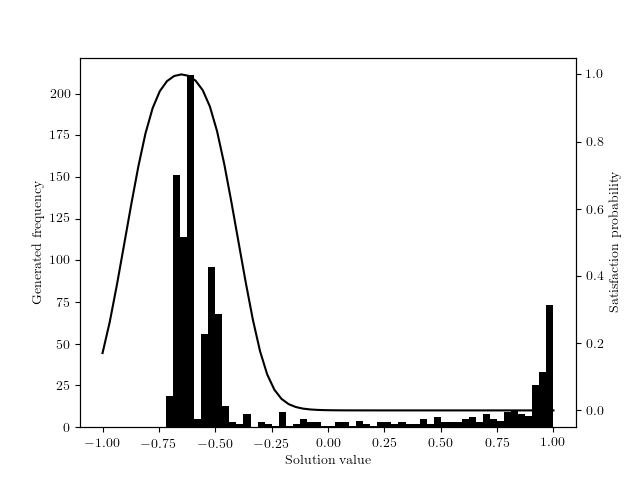
\includegraphics[width=\textwidth]{embeddedConstraint4}
    \caption{
        An example of a constraint whose viable space was so small compared to the solution space that the generator was forced to sample poor solutions to prevent penalties from its recall proxy.
        This can be prevented by reducing the recall proxy weight.
    }
    \label{fig:embeddedConstraintTooSparse}
    \end{center}
\end{figure}
\begin{figure}[H]
    \begin{center}
    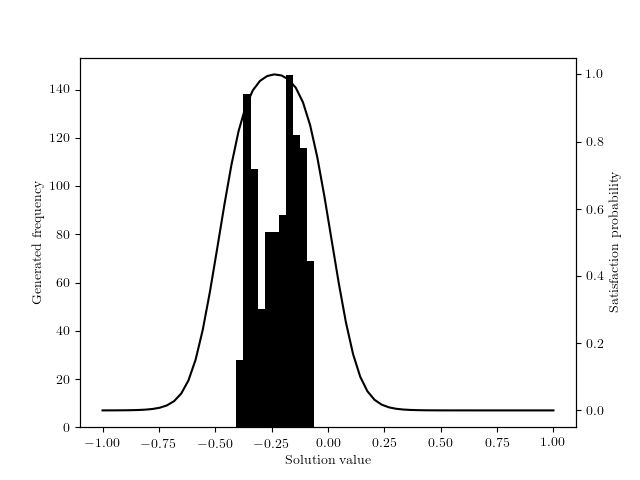
\includegraphics[width=\textwidth]{embeddedConstraint7}
    \caption{
        A constraint for which two peaks join together into a single peak, which is accurately accounted for in the learned viable distribution.
    }
    \label{fig:embeddedConstraintJoinedModes}
    \end{center}
\end{figure}

\section{Method properties}

The first half of this chapter described experiments performed on abstract, simplified engineering problems to inform the design of the project's deliverable architecture.
The remainder of this chapter will examine that architecture's performance in more depth and in more concrete engineering environments.

\subsection{Expected satisfaction probability}

One crucial requirement of the generator is that the solutions it produces should generally have a high satisfaction probability.
The expected satisfaction probability will be used to measure the performance of the generator on various environments, and is calculated by taking the mean across the satisfaction probability, according to $h(c,s)$, of each solution in a sample.
Similarly, the median satisfaction probability is the median of the satisfaction probability of every solution in the sample.

\subsection{Relative density of true solutions}

Another requirement of the generator is that it samples from the entire range of viable solutions.
In all further experiments, identity spread is used as a subtitute for the recall due to its intractibility.
For the purposes of evaluating the generator, the relative density of true solutions in the learned viable distribution will be calculated.

Calculating this value requires a sample of solutions from the true viable distribution: this is achieved by fixing the constraint vector, and then sampling from the discriminator using the Metropolis-Hastings algorithm.
The sampled data should be distributed in approximately the same way as $V(c)$ for sufficiently long Markov chains.

Finding the relative density of each of these solutions in the learned viable distribution requires creating an histogram from a large number of samples from the generator (for $m>1$ an $n$-tree is used to adaptively reduce the number of bins needed).
For each true solution sampled from the Markov chain, the smallest bin within the $n$-tree containing that solution is found.
The relative density of that solution is then defined as the ratio of proportion of generator-sampled points in that bin to the proportion of the volume of the solution space which is bounded by that bin.

Intuitively, if a solution has a relative density greater than $1$ then it is being sampled more frequently than it would be if the generator simply output a uniform distribution; conversely, a relative density of less than $1$ suggests it is being sampled less frequently.
For a generator with good recall it could therefore be expected that the mean relative density over a sample of points taken from the true viable distribution by a Markov chain Monte Carlo algorithm should be above $1$.

\subsection{Data collection}

All environments used in further experiments implemented a common interface that allowed the training of a generator upon them to output a large JSON file containing data about the experiment parameters and results.
An exemplar JSON file is shown in the appendix, but the results were not reproduced here in full due to their excessive size.
Unless otherwise stated: the generator consists of two hidden layers with 4 leaky-ReLU units and a single tanh output unit; the weight and bias constraint embedder also have two hidden layers with 4 leaky-ReLU units and 2 leaky-ReLU output units; pretraining is performed to minimise $q_\text{id}$ and then full training is performed to minimise a weighted sum of the precision proxy and $q_\text{id}$, both until convergence.

\subsection{Effect of recall weight}

A generator was trained on a more concrete engineering environment to examine the effect of tuning $w$ on the tradeoff between precision and recall.
It is hypothesised that low $w$ causes high satisfaction probability but low relative density, whereas high $w$ causes the opposite.

The engineering environment consists of a square plate with sides two units long whose origin is at its centre.
Two holes are drilled into the plate, each described by the coordinates of their centre (which may be anywhere on the plate) and their radius (which may be in $[0,1]$).
One of the hole's parameters are fixed; this hole is taken to be the constraint.
The other hole's parameters are varied as the parameters of the solution.
Satisfaction of the constraint occurs when the holes do not overlap.
As such, $m=n=3$.

Datasets of 64, 256, and 1024 $(s,c,h(c,s))$ tuples were created to train the discriminator, each balanced such that roughly half of the examples satisfied the constraint.
Samples were taken uniformly from $S$ and $C$, and the satisfaction probability was calculated for each pair.
One hidden layer of four leaky-ReLU nodes was used for the discriminator.

\subsection{Equality constraints}

\section{Latent space visualisation}

\end{document}
